\chapter{Algorithme 2}

\section{Présentation}

Le deuxième algorithme reprend le premier algorithme mais décompose chaque rayon entre deux points de surface (ou émetteur/récepteur) en plusieurs segments afin de prendre en compte l'in-scattering provenant de la source (et uniquement de la source) à plusieurs endroits dans la fumée.

\section{Intégration continue}

Prenons un rayon qui après un rebond sur une surface au point $x_i$, repart dans une direction $\omega_i$ pour arriver au point $x_{i+1}$. Alors la luminance arrivant sur le point $x_{i+1}$ et portée par ce rayon est donnée par (eq. \ref{eq:equation_of_transfert}) :
\large \begin{equation*}
    L_i(x_{i+1}, \omega_i) =
        T_r(x_i \longrightarrow x_{i+1})
        L_o(x_i, \omega_i)
        +
        \int_0^t
            T_r(x_i\longrightarrow p')
            L_s(p', \omega_i)
        dt'
.\end{equation*} \normalsize \newline\par

Dans notre cas, nous n'avons pas de lumière émise par la fumée. Seul l'in-scattering intervient et le terme $L_s$ devient donc :
\large \begin{equation*}
    L_s(p, \omega) =
        \sigma_s(p, \omega)
        \int_{\mathcal{S}^2}
            \rho(p, \omega' \longrightarrow \omega)
            L_i(p, \omega')
        d\omega'
.\end{equation*} \normalsize \par

De plus, les $L_i$ venant des différentes directions $\omega_i$ ne sont pas connues dans un premier temps. La seule direction incidente pour laquelle il est possible d'avoir une valeur (autre que la direction $\omega$) est la direction $\overrightarrow{M_{tx}p_k}$ de la source au point $p_k$. Nous n'avons plus qu'un seul choix de direction incidente, il n'est plus nécessaire d'avoir du Monte Carlo et la source devient donc :
\large \begin{equation} \label{eq:source_algo_1}
    L_s(p, \omega) =
        \sigma_{s}(p, \omega)
        \rho(p, \overrightarrow{M_{tx}p} \longrightarrow \omega)
        L_d(p)
,\end{equation} \normalsize
où $L_d(p)$ est la luminance venant directement de la source :
\large \begin{equation}
    L_d(p) = T_r(M_{tx} \longrightarrow p) L_e(M_{tx}, \omega)
.\end{equation} \normalsize

\section{Découpe du rayon}

Le lumière traversant la fumée va rencontrer de nombreuses particules avant d'arriver sur une surface. Il serait lourd de réaliser autant de calculs qu'il n'y a de particules sur le chemin du rayon, mais d'un autre côté ne réaliser qu'un seul calcul serait très inexact. Il faut donc découper ce rayon en plusieurs points $p_i$ séparés d'une distance à trouver de manière cohérente. Mon rayon, lancé au point $p$ et touchant une surface au point $p'$ est donc décomposé comme le montre la figure \ref{fig:decomposition_rayon}.

\begin{figure}[h!]
\centering
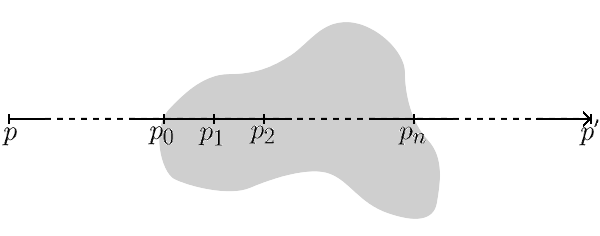
\includegraphics[width=150mm]{ray_decomposition.png}
\caption{Décomposition du rayon}
\label{fig:decomposition_rayon}
\end{figure}

Nous connaissons le point de départ $p$ et le point d'arrivée $p'$ du rayon. Nous pouvons donc connaître le temps $t$ qui correspond à l'arrivée de la lumière sur le récepteur, après avoir effectué le chemin $(M_{tx}, p, M_{r_x})$. Il en va de même pour le temps $t'$ pas le chemin $(M_{tx}, p, p', M_{r_x})$. Avec ces deux données temporelles, il est possible de déduire les positions des points intermédiaires $p_k$, et plus précisément leur distance à $p$, afin d'obtenir des potentiels répartis régulièrement entre $t$ et $t'$, selon une durée $\Delta t$ qui est un paramètre de la simulation. (cf. figure \ref{fig:find_ray_decomposition})

\begin{figure}[h!]
\centering
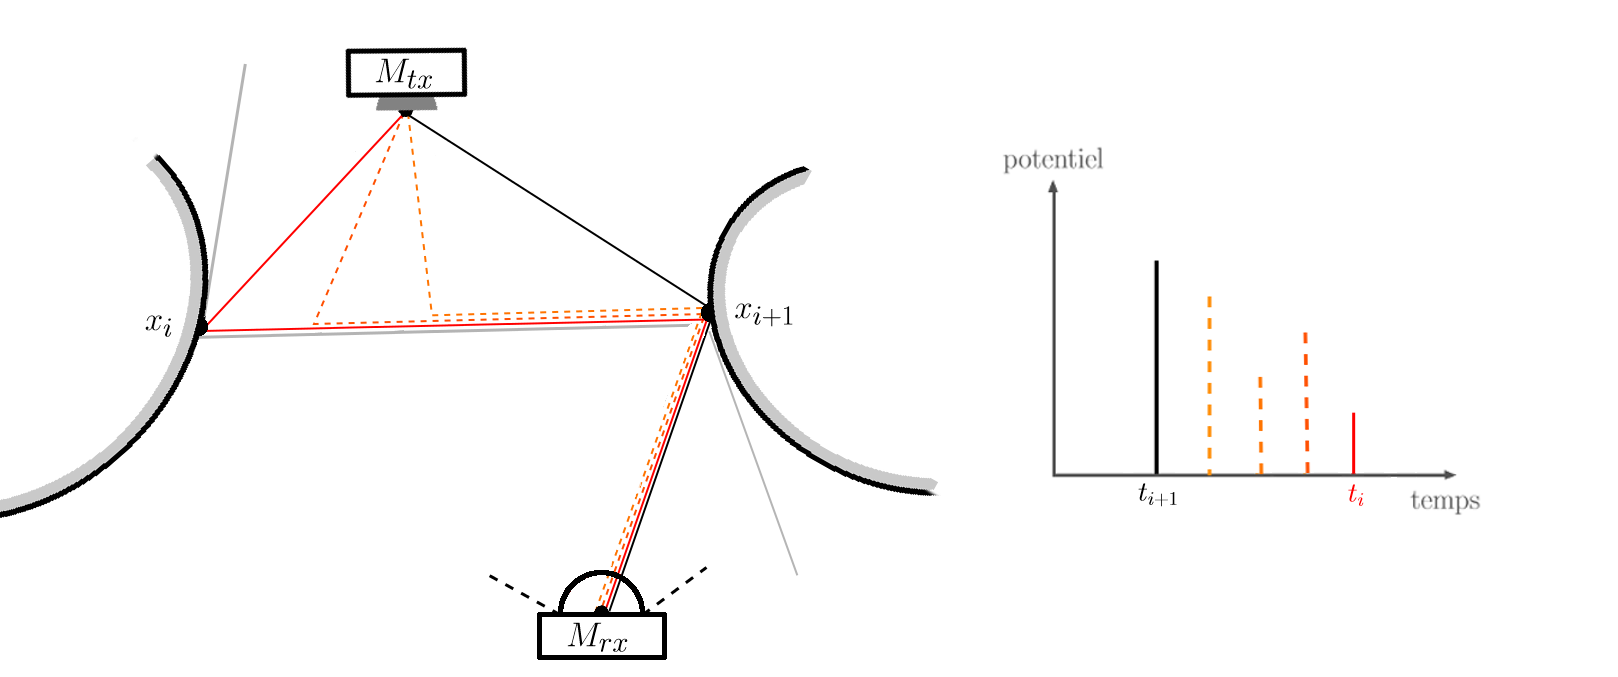
\includegraphics[width=180mm]{find_ray_decomposition_Tx.png}
\caption{Décomposition du rayon et réponse impulsive correspondante}
\label{fig:find_ray_decomposition}
\end{figure}

Pour réaliser la découpe de ce rayon, j'utilise les équations de l'ellipse. En effet, l'inconnue que nous cherchons c'est la distance entre $x_i$ et un point intermédiaire $p$ sur le rayon de direction $\overrightarrow{x_i x_{i+1}}$. Nous connaissons la distance entre $x_i$ et $M_{t_x}$, notons-la $d1$, qui sont des points fixes. Nous connaissons également la longueur totale $L = x_i p + p M_{tx}$, que l'on peut trouver en calculant les temps $t_i$ et $t_{i+1}$. Cette distance étant fixée, nous sommes dans un problème d'ellipse : deux foyers ($x_i$ et $M_{tx}$) et un paramètre (la longueur $L$). Connaissant l'angle $\theta = \angle M_{tx} x_i p$, l'inconnue $r(\theta) = x_i p$ est donc calculable car il s'agit de la distance entre un point de l'ellipse et un foyer, 

\begin{figure}[h!]
\centering
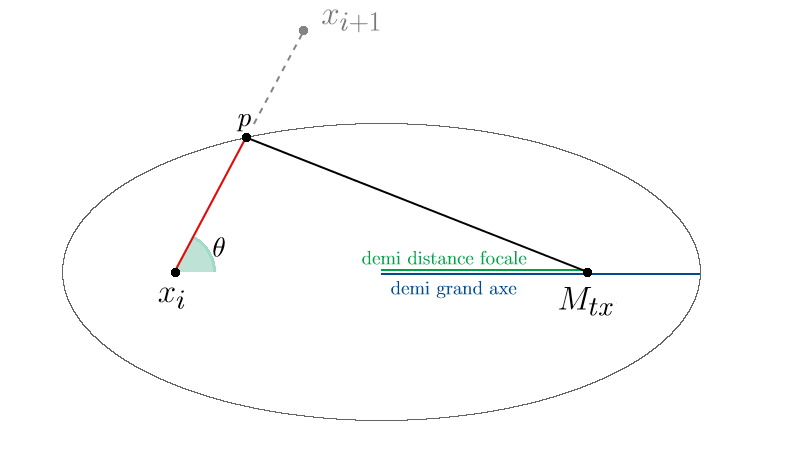
\includegraphics[width=180mm]{ellipseTx.png}
\caption{Utilisation de l'ellipse pour trouver la distance $x_i p$}
\end{figure}

Voici les équations utilisées pour cela :
\begin{itemize}
    \item La longueur du chemin passant par le point $p$ est notée $L = x_i p + p M_{tx}$
    \item La longueur du demi grand-axe est noté $a = L/2$
    \item La distance séparant le centre de l'ellipse et un des foyers, notée $c = x_i M_{tx} / 2$ est la demi-distance focale
    \item L'excentricité est $e = c/a$
    \item Le "paramètre" de l'ellipse est $\gamma = a(1-e^2)$
    \item Enfin, l'équation polaire d'une éclipse nous donne $r(\theta) = \frac{\gamma}{1 + e cos\theta}$
\end{itemize} \par

Ce qui amène l'algorithme suivant :
\begin{lstlisting}[language=java]
private double[] computeStepSizeIn(Ray ray, double stepTime){
    // distance de la source au debut du rayon (de M_tx a x_i)
    double d1 = Ray.createFromFromAndTo(this.irf.transmitter.getPosition(), ray.from).getDistance();
    // distance de la source a la fin du rayon (de M_tx a x_{i+1})
    double d2 = Ray.createFromFromAndTo(this.irf.transmitter.getPosition(), ray.to).getDistance();
    
    // Il va maintenant falloir trouver l'angle theta.
    // Pour cela, on va d'abord chercher la hauteur du triangle (x_i - p - M_tx)
    // en utilisant la formule de Heron
    double perimeter = d1 + d2 + ray.getDistance();
    double p = perimeter/2.0;
    double area = Math.sqrt(p * (p-d1) * (p-d2) * (p-ray.getDistance()));
    double h = area * 2.0 / ray.getDistance(); // la hauteur provenant de la source M_tx
    
    // On peut maintenant trouver l'angle theta avec la formule de trigonometrie suivante :
    // dans un triangle rectangle, nous avons
    // sin(angle) = (longueur du cote oppose)/(longueur de l'hypothenuse)
    // Ici, l'angle theta est celui du sommet x_i
    double theta = Math.asin(h/d1);
    
    // On peut egalement calculer les temsp t1 et t2
    double t1 = d2/physics.getSpeed();
    double t2 = (d1 + ray.getDistance())/physics.getSpeed();
    
    // et en deduire le nombre de points intermediaires qu'il doit y avoir
    // entre x_i et x_{i+1}
    int nbPoints = (int)Math.floor((t2 - t1)/stepTime);
    double[] distancesToRayStart = new double[nbPoints+1];
    
    double[] L = new double[nbPoints+1];
    distancesToRayStart[0] = 0D;
    // pour chaque point, on va pouvoir derouler les equations presentees plus haut
    for (int i = 1; i < distancesToRayStart.length - 1; ++i){
        L[i] = (t1 + i*stepTime) * physics.getSpeed();
    
        // Ellipse
        double a = L[i]/2D; // grand axe
        double c = d1/2D; // demi-distance focale
        double e = c/a; // excentricite
        // utilisation de l'equation polaire
        double A_X = (a*(1-e*e))/(1+e*Math.cos(theta));
        distancesToRayStart[i] = A_X;
    }
    distancesToRayStart[distancesToRayStart.length - 1] = ray.getDistance();
    return distancesToRayStart;
}
\end{lstlisting}

\section{Problème de temporalité}

Je choisis intentionnellement de commencer ma décomposition à l'entrée du milieu participant. En effet, entre $p$ et $p_{0}$, aucune particule ne viendra modifier la radiance et nous avons donc :
$$L_{o}(p, \omega) = L_{i}(p_{0}, \omega).$$\par
De la même manière, à la sortie du milieu participant il ne sert plus à rien de décomposer. Nous aurons :
$$L_{i}(p', \omega) = L_{o}(p_{n}, \omega).$$\par
Bien évidemment, il est tout à fait possible de fusionner $p$ et $p_0$ si dans un premier temps on considère que la fumée remplit toute la scène. Dans ce cas, $p'$ se trouvera aussi dans la fumée et on calculera $L_{i}(p', \omega)$ comme n'importe quel $L_{i}(p_i, \omega)$.

Avec ce que nous savons, nous pourrions décomposer le calcul de la radiance en $n+1$ itérations, en suivant ce schéma :
\large \begin{align*}
L_{i}(p_{0}, \omega) &= L_{o}(p, \omega) ,\\
L_{o}(p_{0}, \omega) &= L_{i}(p_{0}, \omega) - \sigma_{t}(p_{0}, \omega)L_{i}(p_{0}, \omega) + L_s(p_{0}, \omega) ,\\
L_{i}(p_{1}, \omega) &= T_{r}(p_{0}\longrightarrow p_{1})L_{o}(p_{0}, \omega) ,\\
L_{o}(p_{1}, \omega) &= L_{i}(p_{1}, \omega) - \sigma_{t}(p_{1}, \omega)L_{i}(p_{1}, \omega) + L_s(p_{1}, \omega) ,\\
... \\
L_{i}(p_{n}, \omega) &= T_{r}(p_{n-1}\longrightarrow p_{n})L_{o}(p_{n-1}, \omega) ,\\
L_{o}(p_{n}, \omega) &= L_{i}(p_{n}, \omega) - \sigma_{t}(p_{n}, \omega)L_{i}(p_{n}, \omega) + L_s(p_{n}, \omega) ,\\
L_{i}(p', \omega) &= L_{o}(p_{n}, \omega)
.\end{align*} \normalsize\newline\par

Plus généralement, mise à part éventuellement aux extrémités de la décomposition, nous aurions les deux calculs suivants sur lesquels il faudrait itérer (cf. figure \ref{fig:zoom_pk}) :
\large \begin{align}
    \label{eq:deroulement_Li}
    L_{i}(p_{k}, \omega) &= T_{r}(p_{k-1}\longrightarrow p_{k})L_{o}(p_{k-1}, \omega) ,\\
    \label{eq:deroulement_Lo}
    L_{o}(p_{k}, \omega) &= L_{i}(p_{k}, \omega)(1 - \sigma_{t}(p_{k}, \omega)) + L_s(p_{k}, \omega)
.\end{align} \normalsize

\begin{figure}[h!]
\centering
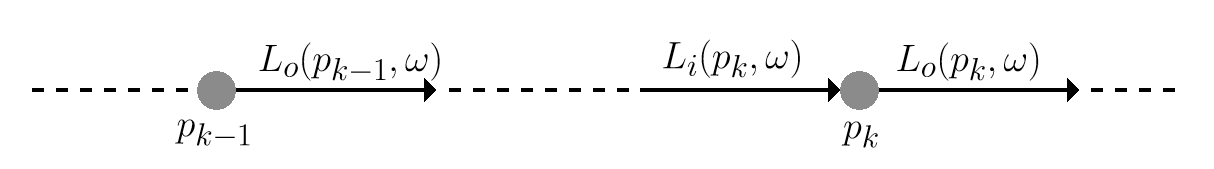
\includegraphics[width=150mm]{zoom_pk.png}
\caption{Zoom sur la décomposition}
\label{fig:zoom_pk}
\end{figure}

Mais il faut prendre en compte que la lumière provenant directement de la source et correspondant à notre in-scattering, ne parcours pas le même chemin que le rayon initialement lancé qui a effectué plusieurs réflexions (figure \ref{fig:different_paths}). Le récepteur ne recevra pas leurs contribution au même moment (figure \ref{fig:different_times}). Il n'est donc pas possible d'itérer comme présenté précédemment puisque $L_s(p_3, \omega)$ ne correspond pas au même pic de potentiel que $L_o(p_2, \omega)$ par exemple.\par
Il faudra compléter la réponse impulsionnelle pour chaque point intermédiaire $p_k$ à des temporalités différentes. Et non pas sommer toutes les contributions, dues à l'in-scattering, sur une même temporalité.

\begin{figure}[h!]
\centering
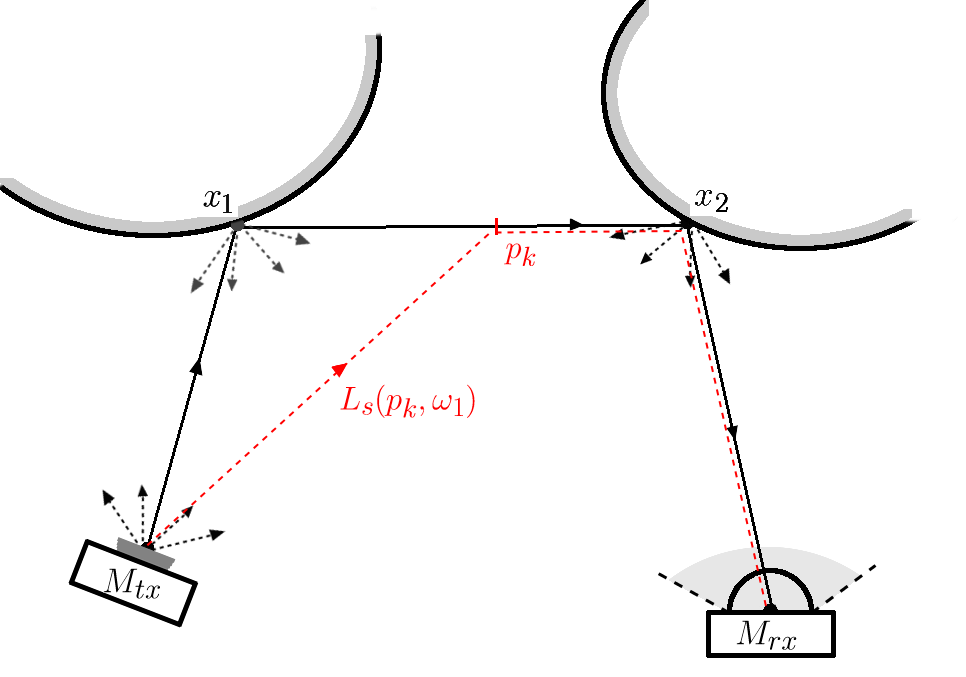
\includegraphics[width=150mm]{time_difference.png}
\caption{Le chemin des réflexions (ligne pleine) est plus long que celui débuté par l'in-scattering (pointillés)}
\label{fig:different_paths}
\end{figure}

\begin{figure}[h!]
\centering
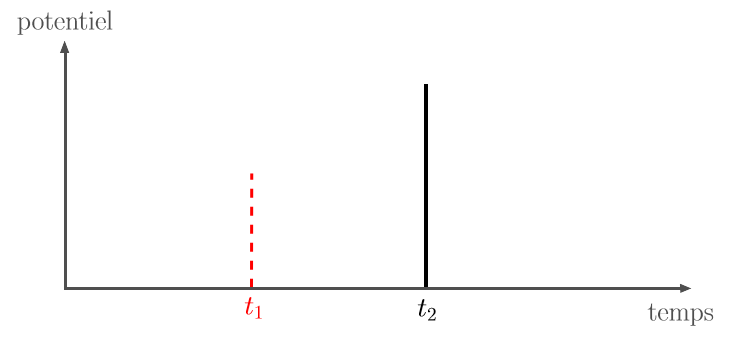
\includegraphics[width=130mm]{potentiel_graph.png}
\caption{La contribution de l'in-scattering est donc reçue plus tôt en $M_{rx}$}
\label{fig:different_times}
\end{figure}

\newpage

\section{Algorithme}

Dans ma classe \textit{\textbf{ParticipatingMedia}}, j'ajoute une méthode qui sera utilisée pour trouver la réponse impulsionnelle finale.

\paragraph{inScatteringAlongARay} Cette méthode calcule la contribution de la source en plusieurs points le long du rayon de direction $\omega$ : c'est l'in-scattering. Pour chaque point intermédiaire $p_i$ (appelons-les \textit{point de milieu} en opposition aux \textit{points de surface}, je calcule la source grâce à la fonction de phase appliquée au point $p_i$ sur le rayon $\omega$. Je multiplie cette source $L_s(p_i, \omega)$ par la transmittance car elle passe également dans la fumée avant d'atteindre le point $p_i$. Puis finalement, j'ajoute cette contribution lumineuse à la réponse impulsionnelle qui sera réutilisée dans une nouvelle itération de la méthode \textbf{RayLaunching}. \newline\par

J'utilise toujours la méthode suivante :

\paragraph{multiplyByTransmittance} Cette méthode ne s'occupe pas de l'in-scattering mais de l'extinction le long du rayon. Puisque ceci correspond au trajet de base du rayon (entre deux points de réflexions trouvé dans la méthode \textbf{RayLaunching}), il n'y a pas besoin de s'occuper de la réponse impulsionnelle ici. En effet, ceci est déjà géré dans la méthode \textbf{RayLaunching}. \newline\newline\par

Il aura également fallut que je modifie la classe \textit{\textbf{ImpulseResponse}} en y ajoutant deux méthodes.

\paragraph{addTime} Après avoir calculé une réponse impulsionnelle potentielle comprenant tout l'in-scattering entre deux points de réflexions $x_i$ et $x_{i-1}$, l'algorithme réalise un rebond vers un autre point de réflexion $x_{i+2}$. Ce nouveau rayon est une distance supplémentaire parcourue par les contributions d'in-scattering sur tous les rayons précédents. Il faut donc, dans la réponse impulsionnelle potentielle, décaler tous les champs en fonction de cette nouvelle longueur. Cette méthode prend donc en paramètre un temps. Il s'agit de la distance du nouveau rayon obtenu après rebond, divisé par la vitesse de la lumière. Et met à jour la réponse impulsionnelle.

\paragraph{addDepth} De la même manière, lorsque ce rebond est effectué, la distance du chemin augmente mais le nombre de réflexions également. L'in-scattering, lorsqu'il est calculé sur le rayon de direction $\omega_i$, est ajouté à une profondeur de 1 puisqu'il ne correspond à aucune réflexion (il vient directement de la source sur un point de milieu sur le rayon), et ceux peut importe le rayon $\omega_i$ sur lequel on travaille. A chaque rebond, il faut donc indiquer que ces contributions ajoutées préalablement dans la réponse impulsionnelle potentielle, effectuent un rebond de plus.


\section{Résultats}

Incorrects pour l'instant. Travail en cours.